\documentclass[11pt, a4paper]{article}

\usepackage{amsmath}
\usepackage{amsfonts} %Matheschriften
\usepackage{amssymb} %Mathesymbole
%\usepackage{mathptmx} % Einstellung für Schriften und Sonderzeichen in mathematischen Umgebungen
                        % ändert SChriftfont
\usepackage{wasysym} % Stellt diverse Sonderzeichen bereit
\usepackage{siunitx}
\usepackage{float}
\usepackage{microtype}
\usepackage{graphicx}
\usepackage{hyperref}
\usepackage{xcolor}
\usepackage[section]{placeins}
% allows for temporary adjustment of side margins
\usepackage{changepage}
\usepackage{rotating}


\usepackage[ngerman]{babel}
\addto\captionsngerman{%
 \renewcommand{\abstractname}{Einleitung}}

\title{Versuch 1: Eigenschaften des Elektron}
\author{Team 2-13: Jascha Fricker, Benedict Brouwer}
\begin{document}
    \maketitle


    \tableofcontents

    \newpage

    \section{Einleitung}

    Bei diesem Versuch werden die Eigenschaften des Elektrons betrachtet und dazu zwei Experimente durchgeführt. Zunächst wird duch das Fadenstrahlrohr
    der Quotient $\frac{e}{m}$ (spezifische Elektronenladung) berechnet. Durch den Millikan-Versuch kann anschließend die Elementarladung $e$ bestimmt
    werden, sodass auch die Masse des Elektrons $m_e$ berechnet werden kann.

    \section{Bestimmung der spezifischen Elektronenladung}

    \subsection{Theorie}

    Im Fadenstrahlrohr werden die Elektronen durch ein elektrisches Feld beschleunigt und durch ein Magnetfeld zu einem Ring abgelenkt. Die Endgeschwindigkeit kann durch gleichsetzten der Energien bestimmt werden, unter der Annahme, dass keine Verluste entstehen

    \begin{align}
    \frac{mv^2}{2} = E_{kin} &= E_{elek} = q \cdot U \label{geschw}\\
    \Rightarrow v &= \sqrt{\frac{2qU}{m}} \,.
    \end{align}
    
    Das Magnetfeld $B$ der Helmholzspulen kann mithilfe der Biot-Savart-Gesetzes bestimmt werden.
    Mit dem Strom $I$, der Windungszahl $N$ und dem Radius $R$ ergibt sich für diesen Versuch

    \begin{align}
        B = \frac{\mu_0 N I}{R} \cdot \left(\frac{4}{5}^{\frac{3}{2}}\right) \label{B-Helm} \,.
    \end{align}

    Die spezifische Elektronenladung ist der Quotient aus Ladung und Masse $\frac{e}{m}$.
    Diese kann durch die Messung des Radius des Strahls im Fadenstrahlrohr bestimmt werden. Es gilt:

    \begin{align}
        \frac{mv^2}{r} = F_{rot} &= F_{mag} = q \cdot v \cdot B \\
        \overset{\text{(\ref{geschw})}}{\Rightarrow} \ \  \frac{q}{m} &= \frac{2U}{B^2 \cdot r^2} \label{qm_formel}
    \end{align}

    \subsection{Ergebnisse}
    \paragraph{Vorüberlegungen}

    Aus einer Beschleunigungsspannung von maximal $300 \si{V}$ kann die maximale Geschwindigkeit eines Elektrons mit Ladung $e$ im nichtrelativistischen Fall
    \begin{align}
        v = \sqrt{\frac{2 e U}{m_e}} = 1,02 \cdot 10^{7} \si{m/s} < 2,9 \cdot 10^{7} \si{m/s} = 10\% \cdot c
    \end{align}


    berechnet werden. Da diese kleiner als zehn Prozent der Lichtgeschwindigkeit ist, kann auch im weiteren nichtrelativistischen gerechnet werden
    Jetzt muss noch überprüft werden, ob die thermische Energie der Glühkathode die Messungen verfälschen könnte.
    \begin{align}
        v_{tmax} &= \frac{v_{100V}}{100} = \frac{\sqrt{\frac{2 e \cdot 100 \si{V}}{m_e}}}{100} = 59310 \si{m \per s} \\
        E_{tmax} &= \frac{m_e \cdot v_{tmax}^2}{2} = 1,602 \cdot 10^{-21} \si{J} = \frac{3}{2} k T_{max} \\
        \Rightarrow \ T_{max} &= \frac{2 E_{tmax}}{3 k} = 77K
    \end{align}
    Die thermische Energie plus die Austrittsarbeit muss kleiner als $E_{tmax}$ sein, da sonst die Messungen verfälscht würden. Wenn die Austrittsarbeit $0$ ist, dann dürfte die Temperatur maximal 77K betragen. Da die Austrittsarbeit des Material aber $\gg0$ und leider nicht bekannt ist, kann die eigenlich maximale Temperatur aber nicht bestimmt werden.


    \paragraph{Auswertung der Messungen}
        Zur Bestimmung des spezifischen Weiderstands wurden zwei Messreihen a 30 Durchführung jeweils mit konstantem B-Feld bzw. konstanter Beschleunigungsspannung mit unterschiedlichen Kreisradien aufgenommen.
        
        Die Ergebnisse der einzelnen Messreihen wurden in der Tabelle \ref{tab:einzelmessungen} ausgegeben.
        \begin{table}[H]
            \centering

            \begin{tabular}{c | c | c | c}
                Radius &  $30 \si{mm}$ in $\si{\coulomb\per\kilogram}$ & $40 \si{mm}$ in $\si{\coulomb\per\kilogram}$& $50 \si{mm}$ in $\si{\coulomb\per\kilogram}$ \\ \hline
                $I = 1,3(1) \si{\ampere}$  & $1.96(44) \cdot 10^{11}$ & $1.76(39) \cdot 10^{11}$ &$1.74(38) \cdot 10^{11}$ \\
                $U = 150(14) \si{\volt}$ & $1.81(30) \cdot 10^{11}$ & $1.79(29) \cdot 10^{11}$ &$1.84(30) \cdot 10^{11}$ \\
            \end{tabular}
            \label{tab:einzelmessungen}
            \caption{Einzelmessungen}
        \end{table}
        
        Daraus folgt als Endergebnis: 
        \begin{align}
            \frac{e}{m_e} &= 1.81(14) \cdot 10^{11} \frac{\si{\coulomb}}{\si{\kilogram}} \label{emend} \\
            \text{Literaturwert:} \ \ \frac{e}{m_e} &= 1,7588 \cdot 10^{11} \frac{\si{\coulomb}}{\si{\kilogram}}
        \end{align}

        Der Literaturwert liegt also im Konfidenzintervall der Messung und die Abweichung ist für diese Messmethode sehr gut. \\
        Die Messdaten wurden durch den gewichteten Mittelwert \cite[Kapitel 5]{ABW} mit dem zugehörigen internen bzw. externen Fehler für jeden Radius einzelnd gemittelt.
        Mit diesen Mittelwerten lässt sich unter berücksichtigung der gaußschen Fehlerfortpflanzung \cite[(19)]{ABW} mittels Gleichung \ref{B-Helm} und \ref{qm_formel} die spezifische Elementarladung für jeden Radius berechen. Die einzelnen Werte lassen sich abermals mit dem gewichteten Mittelwert zum Endergebnis zusammenfassen und mit dem zugehörigen Fehler angeben.
        Dabei gibt es einige Unsicherheiten zu beachten:
        \begin{table}[H]
            \centering
          

            \begin{tabular}{c | c}
                Messgröße & Unsicherheit \\ \hline
                Stromstärke der Helmholzspulen  & $2.5 \% \pm 0.1 \si{\ampere}$ \cite{vc130} \\
                Beschleunigungsspannung & $ 8\% \pm 8 \si{\volt}$ \cite{vc120}\\
                Strichgenauhigkeit & $\pm 0.5 \si{mm}$ \\
                Ablesegenauhigkeit & $\pm 1 \si{mm}$\\
            \end{tabular}
        \end{table}
        
        

    \paragraph{Einfluss des Erdmagnetfeldes}
        Bei der Bestimmung spezifischen Elementarladung wurde zunächst der Effekt des Erdmagnetfeldes auf den Versuchsaufbau
        vernachlässigt. In Garching bertägt die magnetischen Feldstärke $B_{gar} = 48,7 \si{\micro\tesla}$ \cite[]{magnetic_field} bei einem Inklinationswinkel von $\Theta_{incl,gar} = 64.4\si{\degree}$ \cite[]{magnetic_field}. 
        Daraus folgt eine maximale senkrechete Komponente (in Bezug auf die Kreisbahnen) von 
        \begin{align}
        B_{\bot,gar} = B_{gar} \cdot \cos (\Theta_{incl,gar}) = 21.0 \si{\micro\tesla}
        \end{align}
        Dies würde die von uns gemessenen spezifischen Elementarladung um ca. 0.03 \% beeinflussen was im Vergleich zu anderen
        Fehlerquellen vernachlässigbar ist. 
        Um diesen Effekt nachzuweisen bietet es sich an, den Versuchsaufbau so zu positionieren, dass das Erdmagnetfeld senkrecht zum Elektronenring steht.
        Anschließend wird der Versuchsaufbau um 180 \si{\degree} gedreht um den maximalen Effekt des Erdmagnetfeldes zu messen.
        Zur Abschätzung des Effekts lässt sich $B_{min,gar} = B - B_{gar}$ und $B_{max,gar} = B + B_{gar}$ mit einer Beispielspannung von $ U = 300 \si{\volt}$ in \ref{qm_formel} einsetzen.
        Daraus resultiert eine Differenz in den Radien von $5.5 \si{\milli\metre}$, welche im messbaren Bereich liegt.

    

    \section{Millikan}

    In diesem Versuch werden Öltröpfchen mithilfe eines Elektischen Feldes mit und entgegen der Schwerkraft bewegt. Durch den Einfluss des E-Felds auf die Tröpfchen kann Radius und damit die Ladung der Tröpfchen bestimmt werden.

    \subsection{Theorie}

    Durch vorraussetzen eines Kräftegleichgewichts zwischen Reibungskraft und elektrischer Kraft $\pm$ Gravitationskraft bei gleichförmiger Bewegung erhält man einen Radius
    \begin{align}
        r_0 = \frac{3}{2} \sqrt{\frac{\eta_{Luft} (v_{steig} + v_{sink})}{(\rho_{\ddot{Ol}} - \rho_{Luft}) \cdot g}}%{ \rho_{Öl} - \rho_{Luft} \cdot g }
    \end{align}
    Wobei $\rho$ die Dichte des jeweilligen Stoffes ist und $v_{steig}$ bzw. $v_{sink}$ ist die Geschwindigkeit mit der die Tröpfchen steigen bzw. sinken. Dabei muss $v_{steig}$ negativ sein. Aufgrund der kleinen Größe der Tröpfchen muss die Viskosität mit einem Korrekturterm versehen werden:
    \begin{align}
        \eta_{korr} = \eta_{Luft}\left(1+\frac{A \lambda}{r_0}\right)^{-1}
    \end{align}
    Hier wurden die Werte $A = 1,257$ und $\lambda = 72(2) \si{\nano\metre}$ eingesetzt.
    Auch der Tröpfchenradius muss korrigiert werden:
    \begin{align}
        r_{korr} = \sqrt{r_0^2 + \left(\frac{A \lambda}{2}\right)^2} - \left(\frac{A \lambda}{2}\right)
    \end{align}
    Damit lässt sich die Ladung der Tröpfchen $q$ mit der Angelegten Spannung $U$ und dem Abstand der Platten $d$ bestimmen:
    \begin{align}
        q = \frac{3 \pi d}{U} \cdot \eta_{korr} \cdot r_{korr} \cdot \left(v_{steig} - v_{sink}\right)
    \end{align}
    Wenn alles richtig berechnet wurde, müssten die errechneten Werte vielfache der Elementarladung $e = 1.602 \cdot 10^{-19} \si{C}$ sein.

    \subsection{Ergebnisse}
    Um die Verteilung zu veranschaulichen, wurde im Graphen \ref{fig:milllikam} die Ladung $q$ gegen den errechneten Radius $r_{korr}$ geplottet.
    \begin{figure}[h]
        \centering
        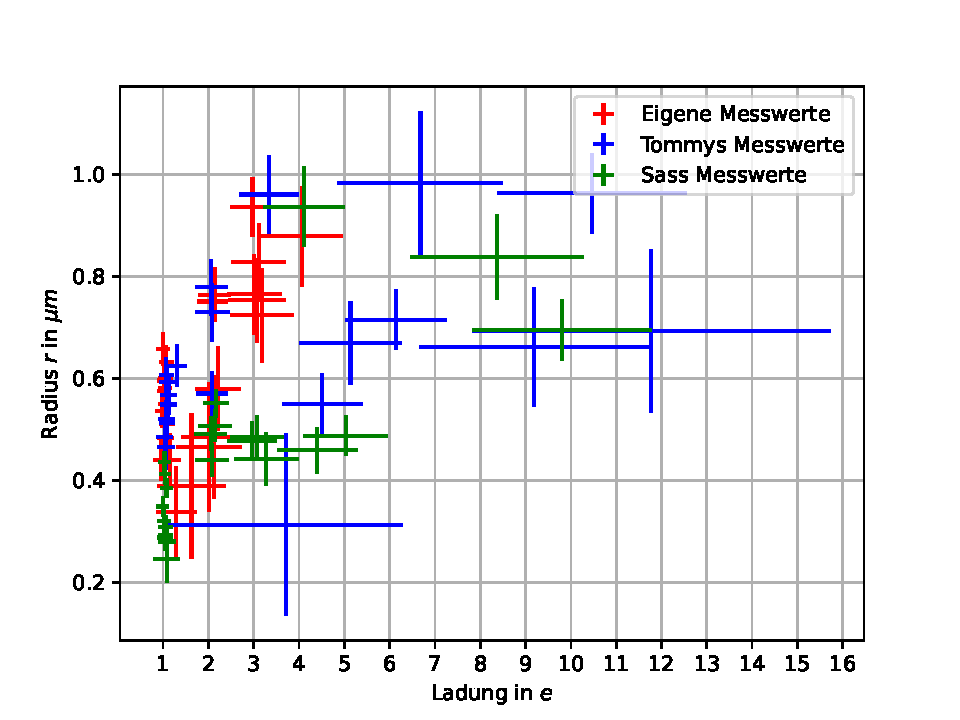
\includegraphics[width=\textwidth]{millikan.pdf}
        \caption{Ladung der Tröpfchen und Radius im Milllikamversuch}
        \label{fig:milllikam}
    \end{figure}
    Außerdem wurde die Häufigkeitsvertielung der Ladungen im Graphen \ref{fig:hauf} ermittelt.

    \begin{figure}[h]
        \centering
        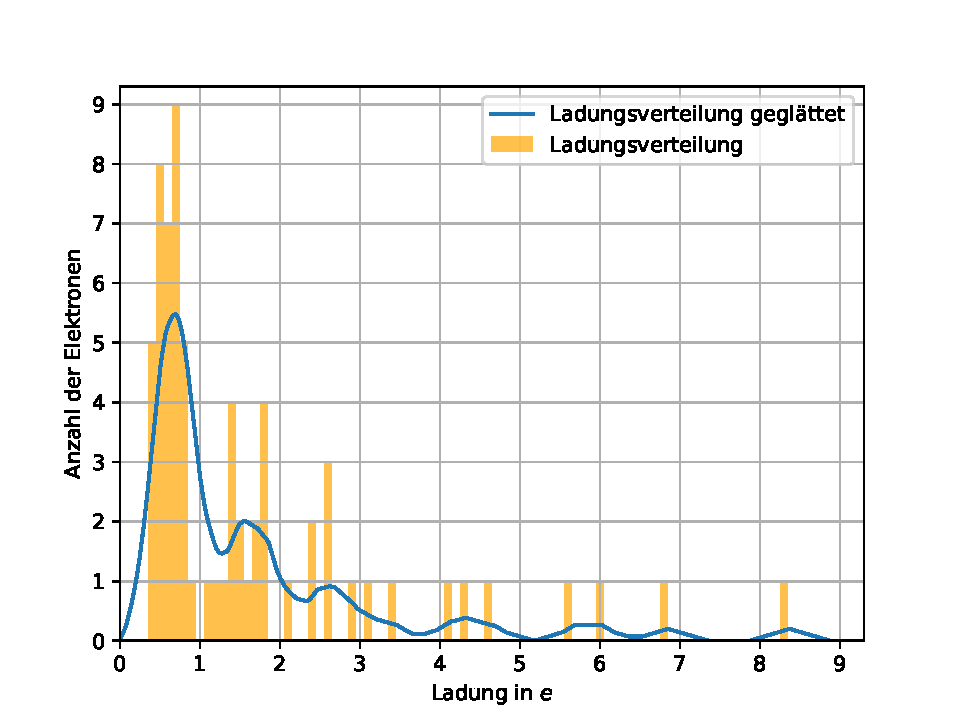
\includegraphics[width=\textwidth]{Ladungsverteilung.pdf}
        \caption{Häufigkeitsverteilung der Ladungen im Millikanversuch}
        \label{fig:hauf}
    \end{figure}
    
    Durch die Position des ersten Maximums kann die Elementarladung grob abgeschätzt werden. Durch diesen Schätzwert lassen sich nun Intervallgrenzen definieren um die Tröpfchen nach Ladungsanzahl zu sortieren.
    Daraus lässt sich die Elementarladung bestimmen, indem der gewichtete Mittelwert zzgl. Fehler berechnet\cite[Kapitel 5]{ABW} wird:
    \begin{align}
        e &= 1,03056(99) \cdot 10^{-19} \si{\coulomb} \\
        \text{Literaturwert:} \ \ e &= 1,602 \cdot 10^{-19} \si{\coulomb}
    \end{align}
    Anhand von diese Berechnung und der Elektonenladung (\ref{emend}) kann die Masse der Elektrons berechnet werden:
    \begin{align}
        m = e \cdot \left(\frac{e}{m}\right)^{-1} &= 5,68(43) \cdot 10^{-31}\\
        \text{Literaturwert:} \ \ m &= 9.10938 \cdot 10^{-31} \si{\kilogram}
    \end{align}

    Die in Tabele \ref{unsichmili} angegebenen Unsicherheiten wurden berücksichtigt.
    \begin{table}
        \begin{tabular}{c | c | c}
            Messgröße & Beschreibung & Unsicherheit \\ \hline
            Spannung $U$ in $\si{\volt}$ & 1 Digit = 1V & $u_U = \frac{1}{2\sqrt{3}} \si{\volt}$ \\
            Zeit $t$ in $\si{\second}$ & 1 Digit = 0,1s + Reaktionszeit 0,2s & $u_t = \sqrt{\frac{0.1}{2\sqrt(3)}^2 + 0.4} \ \si{\second}$ \\            Abstand $s$ in $\si{\metre}$ & 1 Strich = 0,1mm & $u_s = \frac{0.0001}{4\sqrt{3}} \si{\metre}$ \\
            freie Weglänge $\lambda$ & Siehe \cite{ELE} & $u_\lambda = 2 \si{\nano\metre}$ \\
        \end{tabular}
        \caption{Unsicherheiten der Messwerte}
        \label{unsichmili}
    \end{table}
    Die Werte für Viskosität $\eta_{Luft}$ und Dichte $\rho_{Luft}$ der Luft \cite[]{Luft} sowie Dichte des Öls \cite{ELE} wurden ohne Unsicherheiten benutzt.




    \section{Diskussion}
    Bei der Bestimmung der spezifischen Elementarladung erhielten wir sehr genaue Ergebnisse, bei denen der Literaturwert im Konfidenzintervall liegt. Auch die errechneten Werte beim Millikan-Versuch sind sehr nah an den Literaturwerten dran. Durch den Tipp unseres Tutors konnte der Fehler in der Rechung gefunden werden. Insgesamt konnten trotz der "ungenauen" Messmethoden durch die große Anzahl an Datenpunkten relativ genaue Werte ermittelt werden98
    
    % Im Gegensatz dazu weicht das Ergebniss des Millikan-Versuch um fast 40 \% vom Literaturwert ab, sodass dieser nicht mehr im Konfidenzintervall ist.
    % Dies liegt vermutlich an einer vergleichsweise geringen Anzahl an Versuchsdurchführungen verbunden mit einer ungenauen Messmethode. Außerdem gibt es wahrscheinlich in unserer Auswertung oder im experimentellen Vorgehen weitere systematische Fehler, da sich die Öltröpfchenladung eindeutig um einen fehlerhaften Wert häuft.
    

    \bibliographystyle{plain}
    \bibliography{literature}

\end{document}